\documentclass{report}
\usepackage{graphicx}
\begin{document}
\subsection{Méthode de placement de pièce}

    \paragraph{}L'objectif de cette méthode est de renvoyer l'ensemble des positions possibles pour
    une pièce dans un pattern. Après notre première étude du sujet, nous avons cherché comment nous,
    en tant qu'être humain, nous réalisons cette tâche.  La première approche consistait à tester
    toutes les positions possibles pour une pièce, cependant d'un point de vue programmation ainsi
    que d'un point de vue intelligence cette méthode n'est pas très efficace. 

    \paragraph{} Pour avoir une résolution efficace on a conclut qu'il fallait absolument "coller" 
    les pièces au pattern, mais toujours de manière intelligente. On a donc cherché les points 
    communs entre la pièce et le pattern afin de trouver un point ou une arête constituant la base 
    du placement de la pièce. 
    
    \paragraph{}Le premier point commun est la longueur des arêtes, en effet les pièces du Tangram
    ayant chacune des caractéristiques différentes, si une arête du dessin coïncide avec une arête
    de la pièce, il y a de grande chance pour que la pièce soit positionnée à cet endroit. 
    
    \begin{center}
    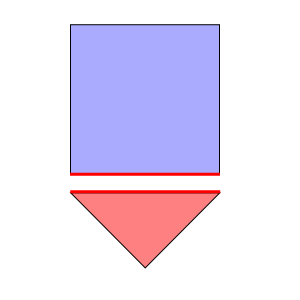
\includegraphics[width=5cm]{place_figure_exacte_match}
    \end{center}

    \paragraph{}Cependant cette méthode a ses limites, il se peut que lors de la résolution de
    celui-ci une arête du pattern corresponde à plusieurs pièces. Lors de ce genre de configuration
    la première méthode est inefficace. 

    \begin{center}
    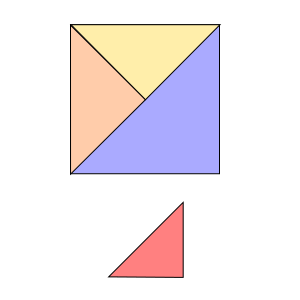
\includegraphics[width=5cm]{place_figure_probleme_exacte_match}
    \end{center}

    \paragraph{}Le second point commun qui va donc nous aider, pour la décision de placement de la
    pièce, est l'utilisation des angles de chaque pièces. Si aucune des arêtes du pattern ne
    correspond, alors il va falloir vérifier si un angle du pattern est égal à l'un des angle de la
    pièce. 

    \begin{center}
    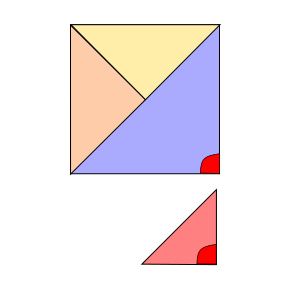
\includegraphics[width=5cm]{place_figure_probleme_angle_match}
    \end{center}

    \paragraph{}Une fois la base du placement de la pièce trouvée, on obtient soit une arête, soit
    un angle composé de deux arêtes. Il faut donc ensuite positionner la pièce en fonction de
    celle-ci à l'aide de translation et rotation. Cependant une fois la pièce correctement placé
    sur le pattern par rapport à la base, il reste le soucis du sens de la pièce. En effet, selon la
    rotation et le sens initiale de la pièce, celle-ci peut se trouver à l'inverse de la position
    voulue. 


    \begin{center}
    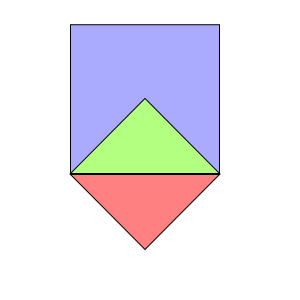
\includegraphics[width=5cm]{place_figure_probleme_symetrie_1}
    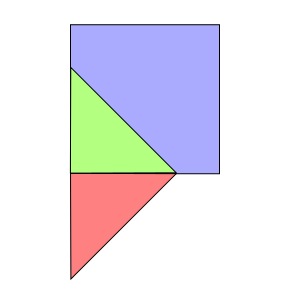
\includegraphics[width=5cm]{place_figure_probleme_symetrie_2}
    \end{center}

    \paragraph{}Ceci nous amène au plus gros problème du positionnement d'une pièce, la validation
    de la position. Après l'obtention d'une position il faut donc vérifier si tous les sommets de la
    pièce font partie de la pièce. Car il ne faut pas que les pièces se superposent, ni qu'elle soit
    à l'extérieur du pattern.

    \begin{center}
    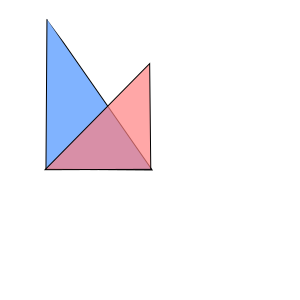
\includegraphics[width=5cm]{place_figure_probleme_point}
    \end{center}

    \paragraph{} Pour résoudre ce problème nous avons utilisé un algorithme qui pour chaque sommet
    de la figure compte le nombre d'arêtes ayant un point à la même hauteur que le sommet et si il y
    a un nombre impaire de point de chaque coté du point alors le point est à l'intérieur du pattern
    sinon à l'extérieur.
    \\ source : http://alienryderflex.com/polygon/

    \paragraph{} Après avoir tester l'ensemble des points de la pièce positionné et de son
    symétrique, fatalement l'une des pièces est en partie à l'extérieur.

    \paragraph{} Le prédicat chargé de générer l'ensemble des placements possibles va donc pour une
    pièce et une figures données, tenter de trouver les positions à l'aide de la première méthode
    puis de la seconde et dans le deux cas va tester la validité des résultats trouvés.
    Dans le cas où aucun placement n'est possible, c'est à dire si le pattern est trop petit pour
    accueillir la pièce ou si aucun angle ni aucune arête ne convient le prédicat va échouer.

\end{document}
